\chapter{Case Study 1: A Component Modelling Language}

\section{Introduction}

The best way to learn how to metamodel is to look at some real
examples. This chapter gives a detailed walkthrough of the
development of a metamodel for a commonly used modelling language:
DFD's. DFD's were widely used in the 1980's and early 1990's as a
notation for modelling the flow of data between entities in a
system. Indeed they are still used today by data modellers as an
important tool for eliciting data structures. DFD's are a good
starting point for illustrating metamodelling as they are simple,
but illustrate many facets of the metamodelling process.

We begin by giving an overview of DFD's and then follow the
chapters in the book in the development of a metamodel, starting
with the construction of an abstract syntax model, an executable
semantic model, and a concrete syntax model. The resulting
metamodel will be sufficiently rich enough to support the
construction of DFD models both graphically and textually. It will
also have a fully operational semantics, enabling DFD models to be
executed by the XMOF virtual machine. In short, a complete tool
description.

\section{Overview}

As shown in figure \ref{dfdexample}, a DFD is essentially a visual
network of data flows between processes, data stores and external
entities, which aims to model the logical flow of data in a system
and the transformations that occur to the data (without committing
to physical implementation details).

\begin{figure}[htb]
\begin{center}
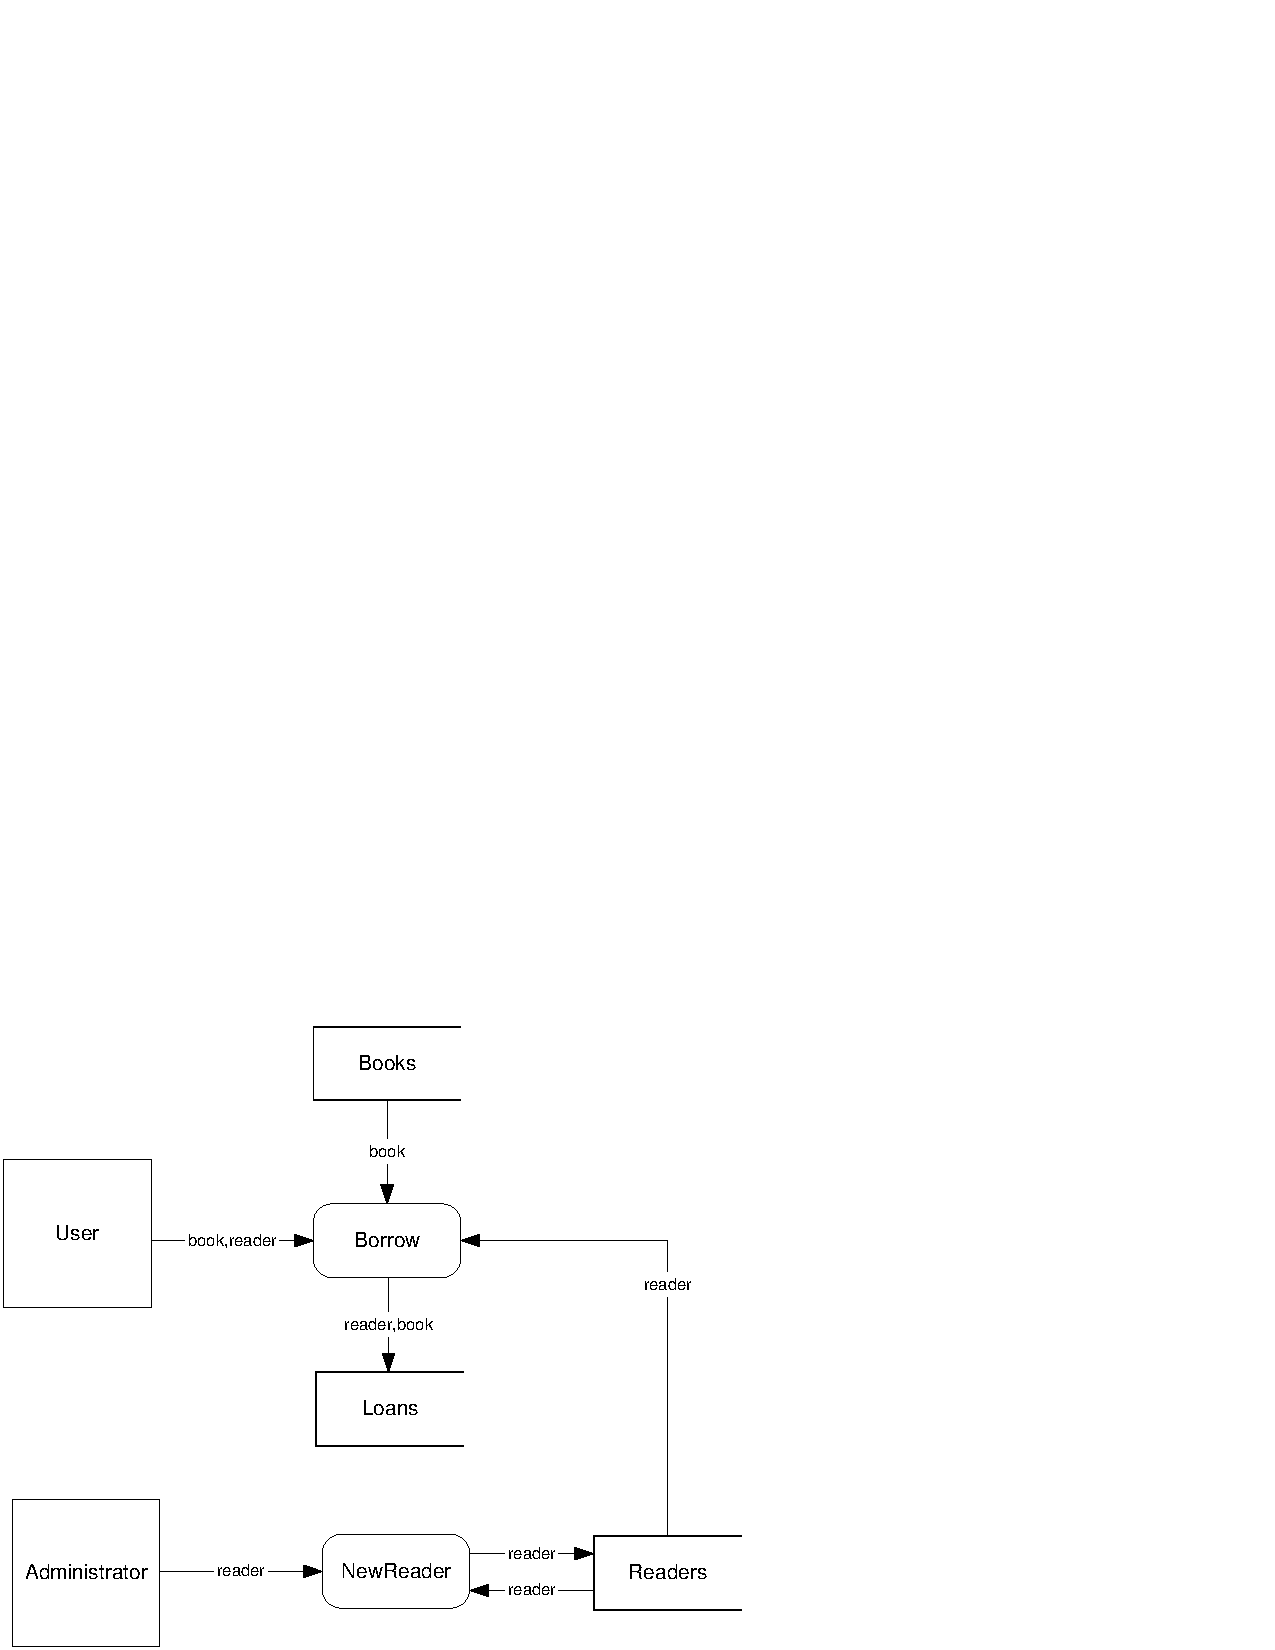
\includegraphics[width=13cm]{CaseStudy1/figures/DFDExample.pdf}
\caption{An example of a data flow diagram (DFD)}
\label{dfdexample}
\end{center}
\end{figure}

There are a number of other features of DFDs that are not
illustrated by this example. One of the most important is the
ability for processes to be nested. As shown in figure
\ref{dfdnested} ,this enables a single process node on a high level
diagram to be expanded to show a more detailed collections of
processes. The highest level process in the DFD hierarchy is
commonly called a context diagram. This provides a view of the
system as a single process, along with the input and output
dataflows that flow to and from the external entities to the
system.

\begin{figure}[htb]
\begin{center}
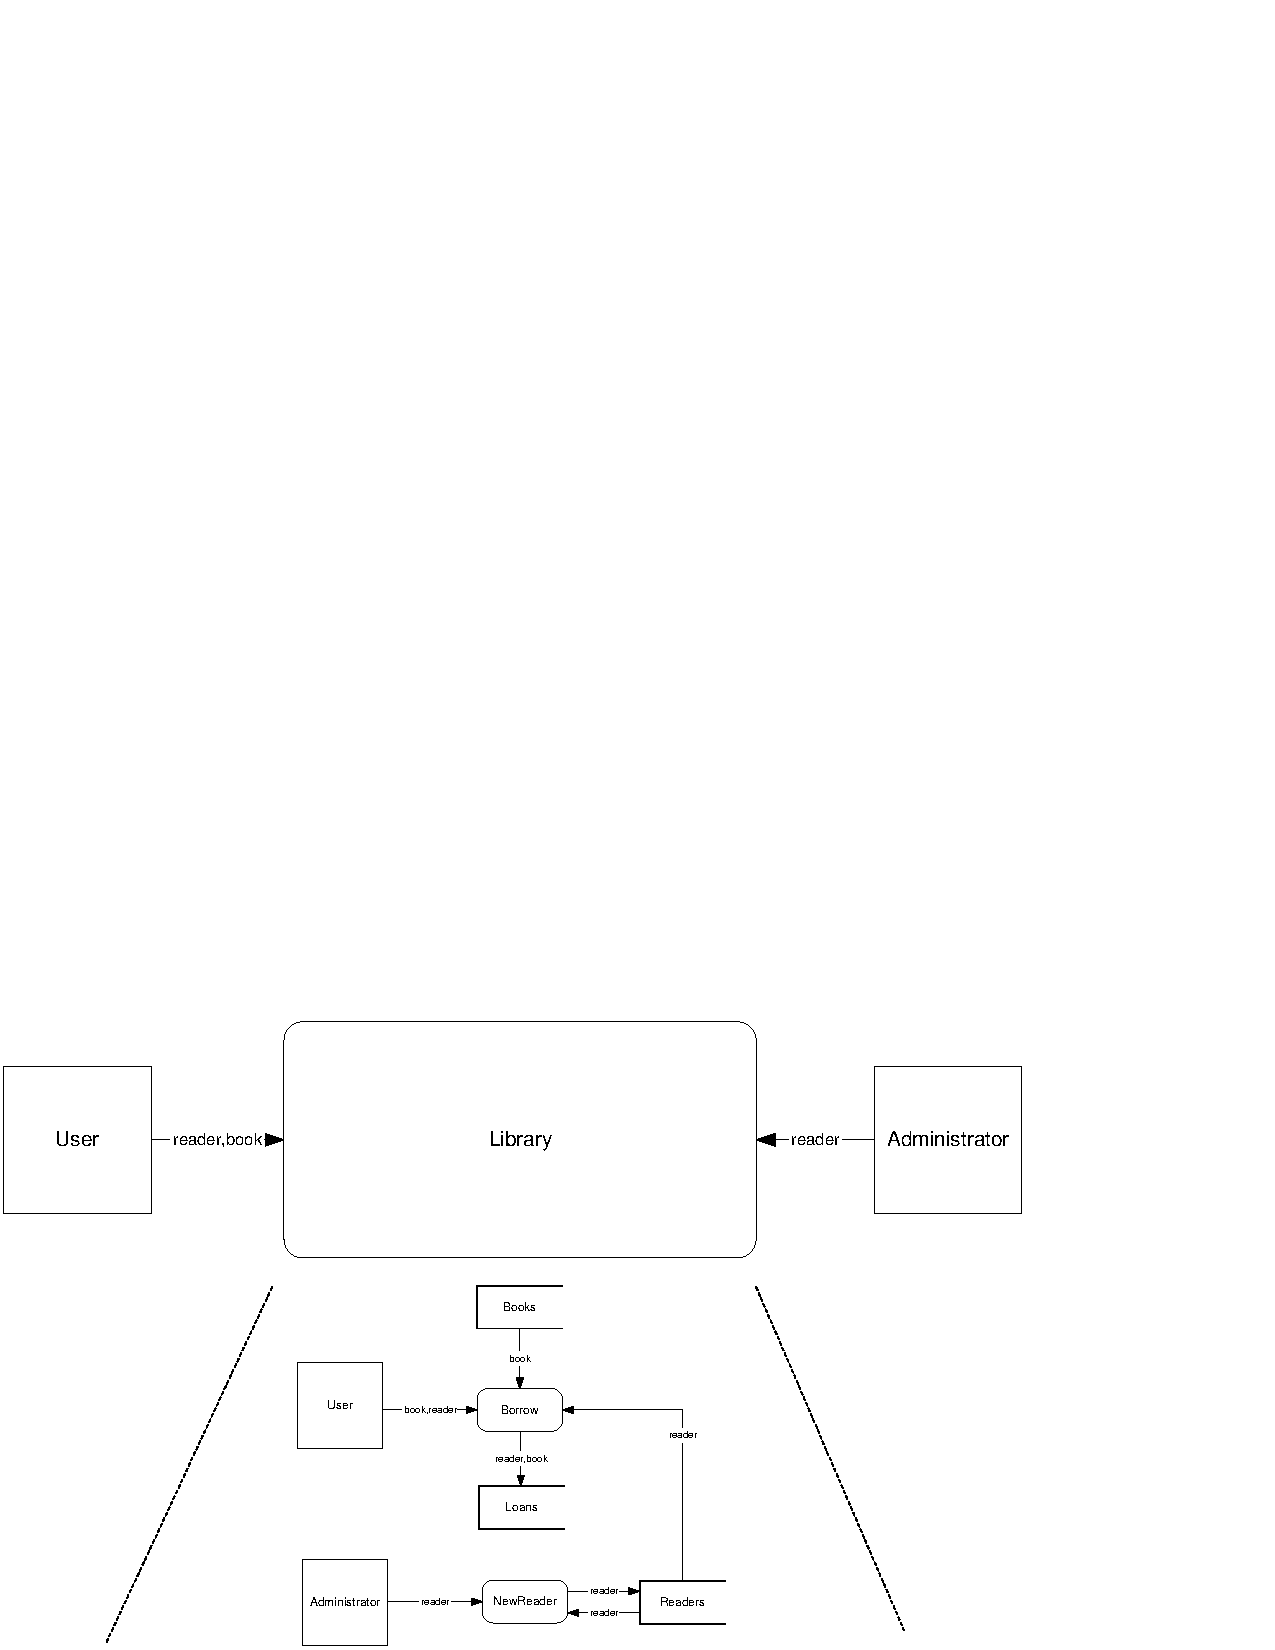
\includegraphics[width=13cm]{CaseStudy1/figures/DFDContext.pdf}
\caption{A nested DFD} \label{dfdnested}
\end{center}
\end{figure}

Processes can be decomposed to any level of detail. The diagram in
figure \ref{addreader} shows the decomposition of the NewReader
process.

\begin{figure}[htb]
\begin{center}
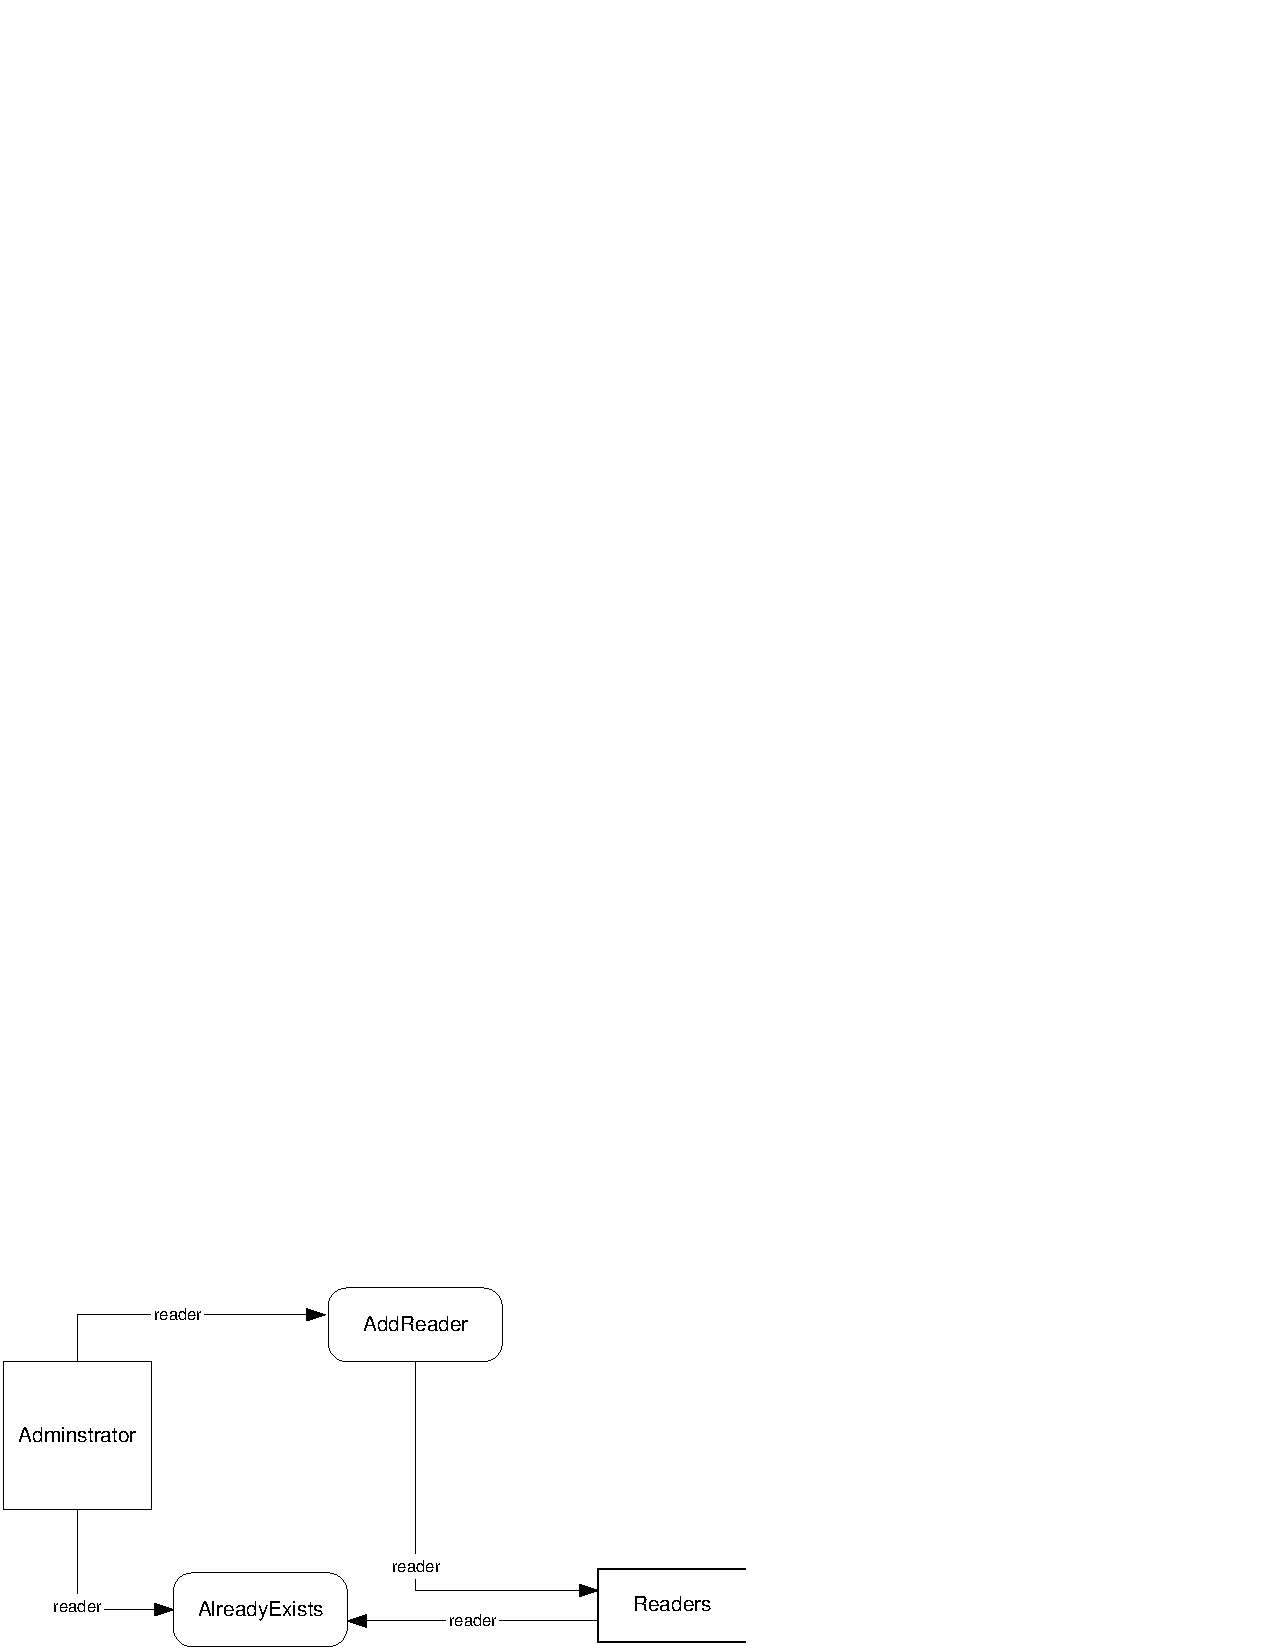
\includegraphics[width=13cm]{CaseStudy1/figures/AddReader.pdf}
\caption{Decomposing the NewReader process} \label{addreader}
\end{center}
\end{figure}

Finally, in order to describe the effect of a leaf process, DFDs
typically provide a simple action language. This can be a
specification style language, such as Pspecs \cite{}, which
describes the effect of the process in terms of pre- and post-
conditions, or it can be an operational language. Because we
ultimately wish to be able to execute the DFD's, the latter has
been chosen.

The action language supports a collection of simple actions for
updating and reading records from datastores, making choices, and
calling other actions in other processes.


\begin{lstlisting}
@Process AddReader(name)
  @When
    not Readers.records->exists(reader | reader->at(0) = name)
  do
    @Block
      @Update Readers with Seq{name} end
      @OCLExp "ReaderAdded" end
    end
  end
end
\end{lstlisting}
The action illustrated here is a When action, which has a
condition, that, if true, results in the activation of the action
in the do expression. In this case, if no reader currently exists
with the same name in the Readers datastore, a sequential Block
action is called. This firstly updates the Readers datastore with a
sequence containing the name of the reader and then produces the
OCL string expression, "ReaderAdded".

\section{Abstract Syntax}

\subsection{Identification of Concepts}

Based on the example shown in figure \ref{dfdexample}, the
following candidates for concepts can be immediately identified:

\begin{description}
\item [Process]  A transformer of information that resides within
the bounds of the system to be modelled. Processes appear as named
circles in a DFD.

\item [External Entity] A producer or consumer of information that
resides outside the bounds of the system to be modelled. An external
entity is drawn as a named box.

\item [Datastore] A repository of data records that is to be stored
for use by one or more processes. A datastore is drawn as a half
open box.

\item [Dataflow] Represents the flow of data between processes,
entities and datastores. Dataflows are named and are uni-directional.
Dataflows are shown as lines with a single arrow at one end, pointing
in the direction of the flow.

\item [Action] An action belongs to a process and has a body which
specifies the effect of the action. The following primitive sets of actions are provided:
\begin{itemize}
\item A Send action causes a process in scope to be activated by sending the process a message.
\item An Update action is used to add a record to a data store.
\item A Remove action removes a record from a datastore.
\item An Or action performs a number of actions in sequence until one of them succeeds.
\item A When action allows actions to be activated provided a condition holds.
\item A Block action contains a sequence of sub-actions, which are activated in order.
\item An OCLExp action that contains an XOCL expression which can be evaluated in the normal way.
\end{itemize}

\end{description}

Figure \ref{dfdannotated} shows the same DFD model 'marked up' with
some of the identified concepts. A similar exercise can be carried
out for elements in the action language example.

\begin{figure}[htb]
\begin{center}
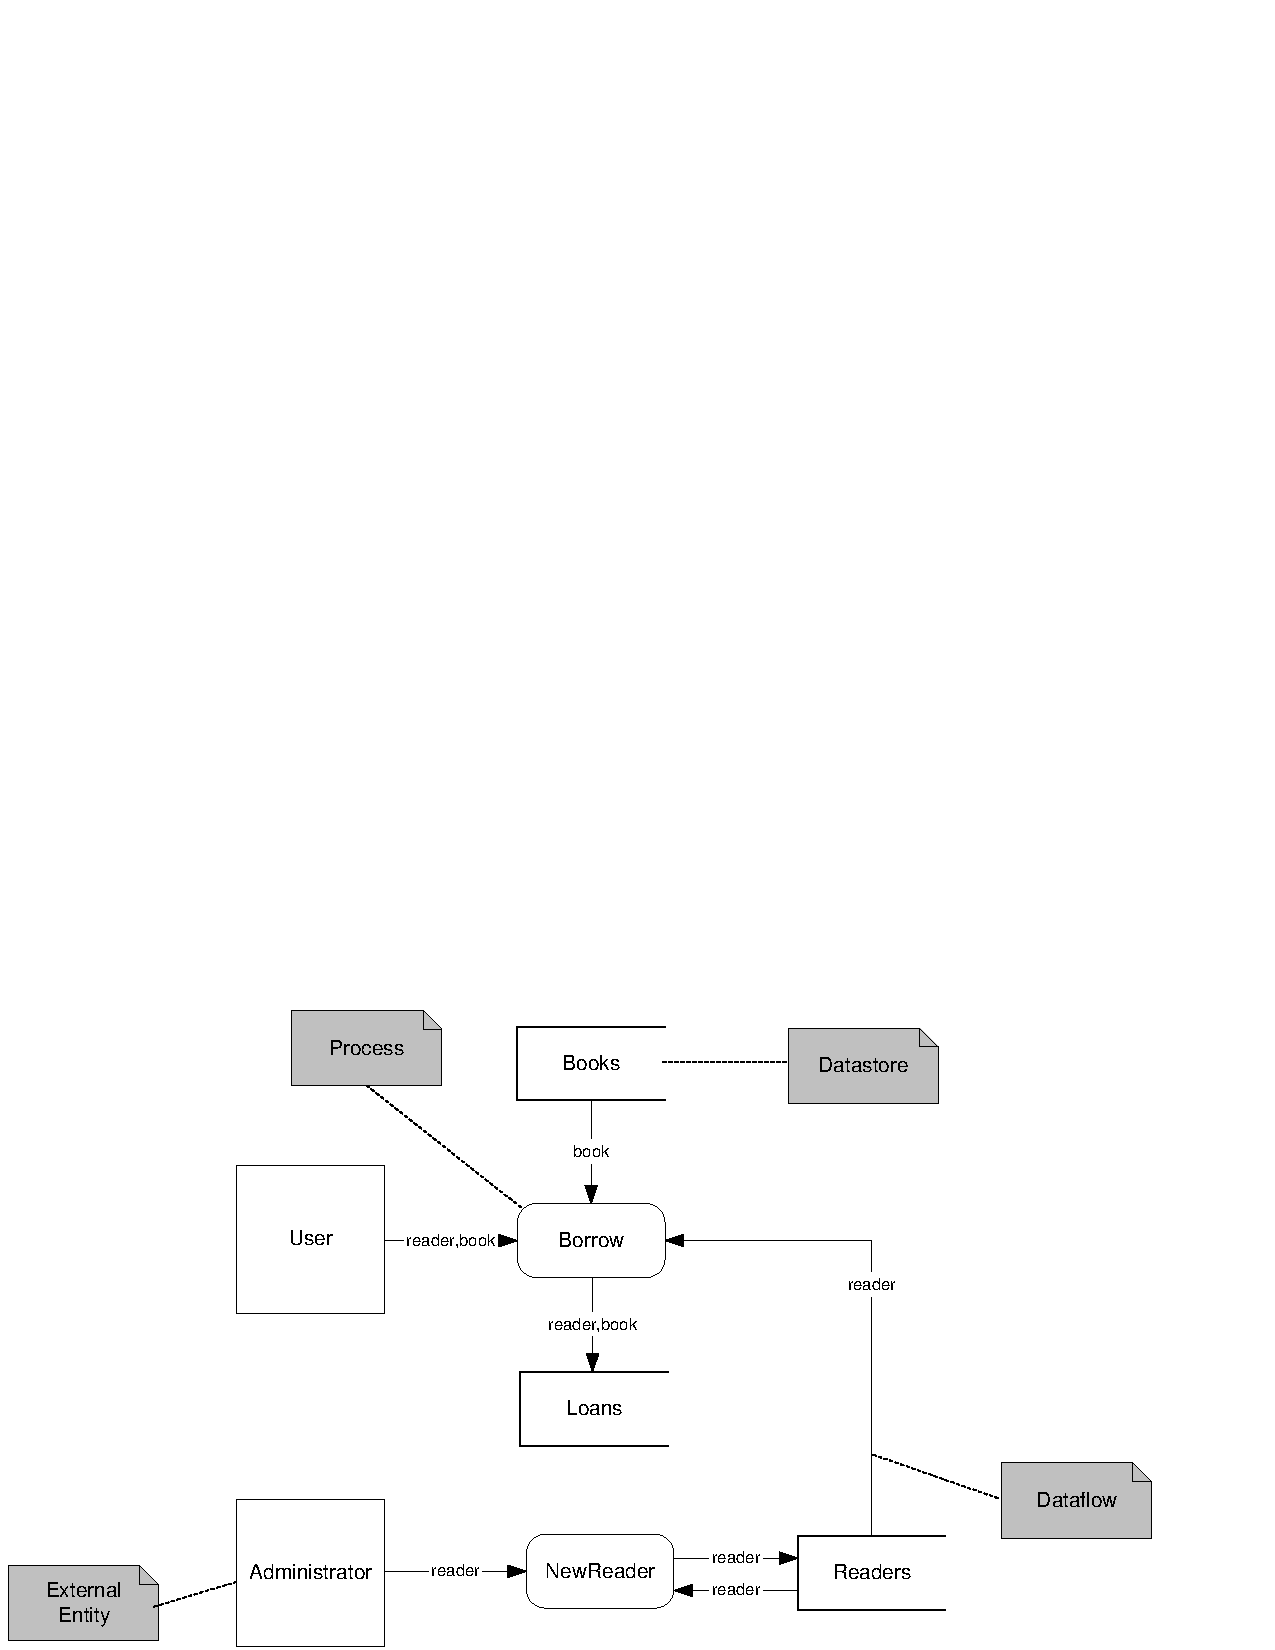
\includegraphics[width=13cm]{CaseStudy1/figures/DFDAnnotated.pdf}
\caption{An annotated example of a data flow diagram (DFD)}
\label{dfdannotated}
\end{center}
\end{figure}

\subsection{Abstract Syntax Model}

Once some candidate concepts have been identified, the next step is
to construct an abstract syntax model.

An important question to ask at this point is whether each concept
is an appropriate abstract syntax concept. Datastores, processes
and actions are clearly core to DFDs, as they capture the central
concepts of data and data transformation. There is a question mark
however over external entities and data flows:

\begin{itemize}
\item External entities are external to the system being modelled,
and would appear to be redundent in the sense that they only add
contextual information.
\item Dataflows appear to be derived concepts, as they could be thought
of as showing information flow dependencies between processes and
datastores as the result of actions. For instance, a flow from a
process to a datastore can be derived from an action belonging to
the process that updates the datastore.
\end{itemize}

\noindent For now, these two concepts will be put to one side
\footnote{They will be considered further in the concrete syntax
chapter}.

By focusing on processes, datastores and actions, the model shown
in figure \ref{dfdabs1} is obtained.

\begin{figure}[htb]
\begin{center}
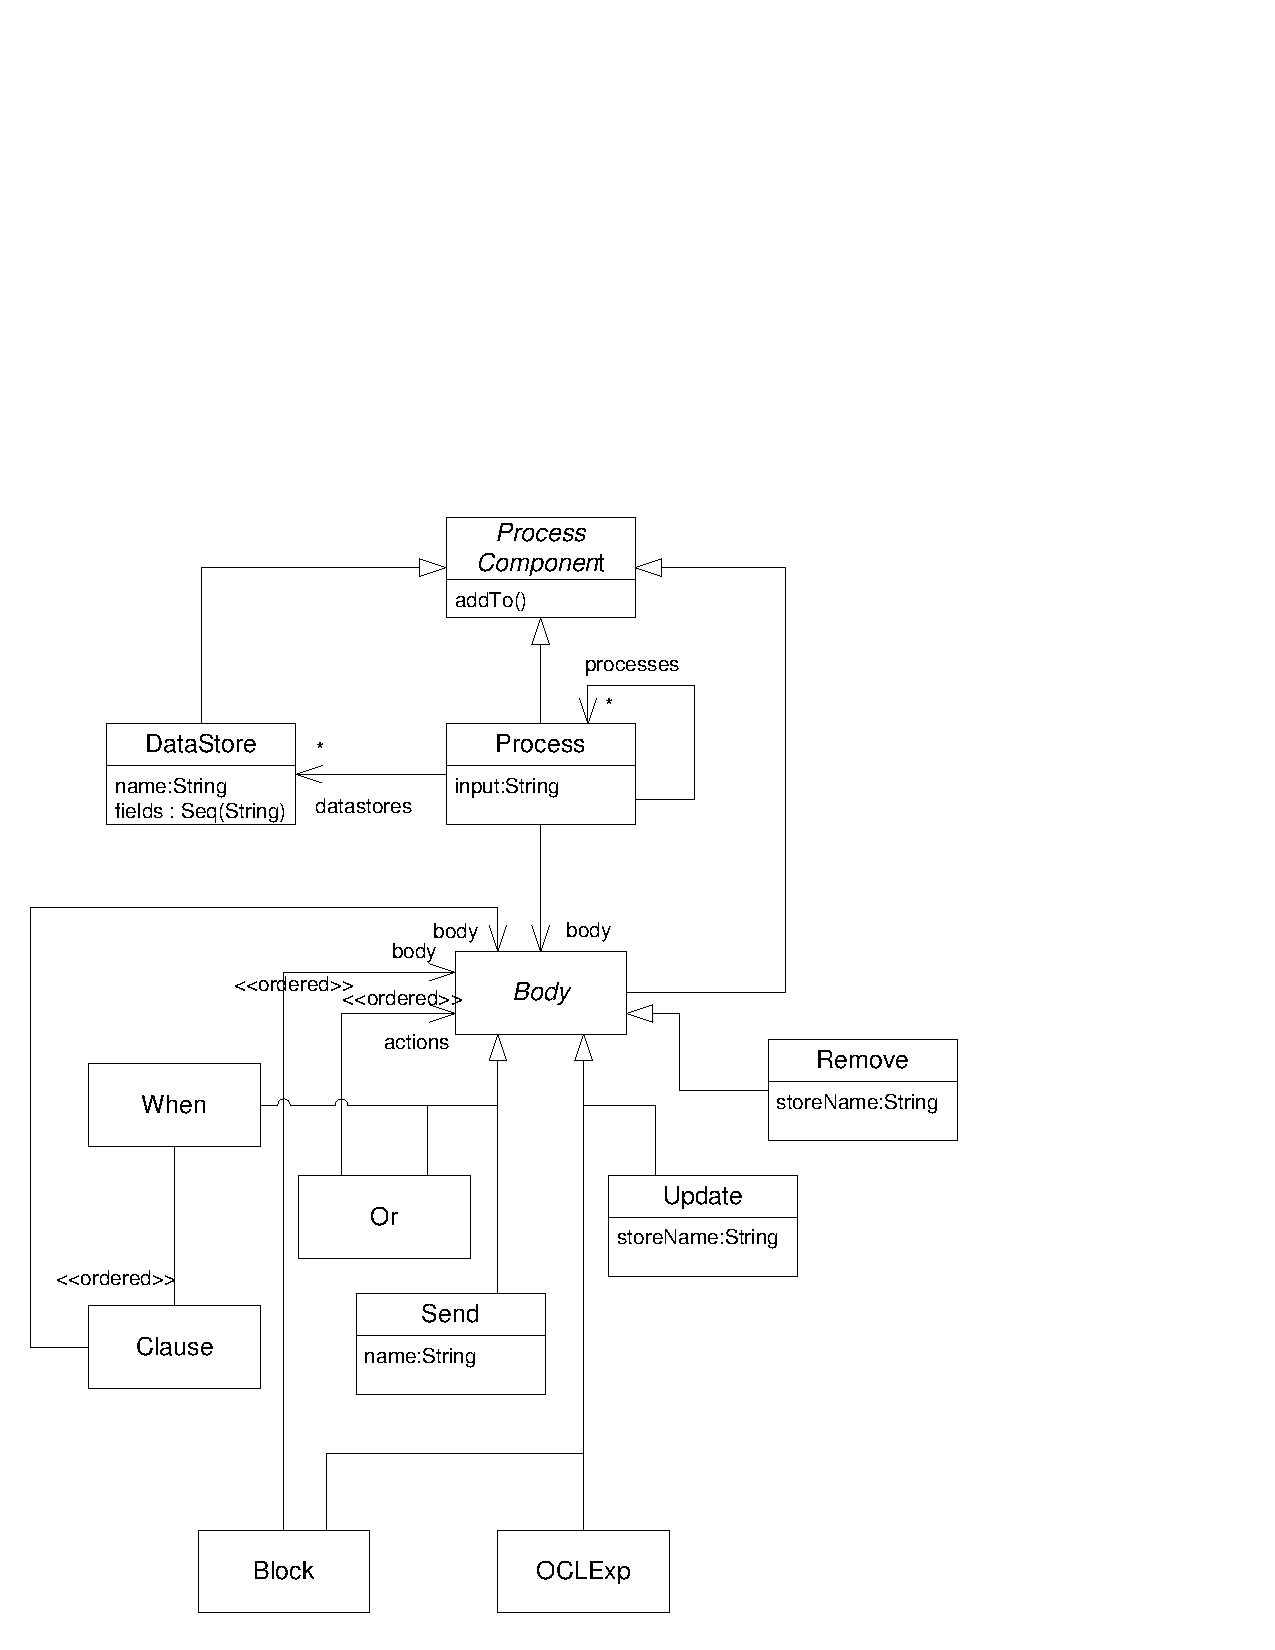
\includegraphics[width=10cm]{CaseStudy1/figures/DFDAbs1.pdf}
\caption{An abstract syntax model for DFDs} \label{dfdabs1}
\end{center}
\end{figure}

There are a number of points to note about the model:

\begin{itemize}
\item Processes are associated with: the collection of datastores that
are accessible by the process; a single action body; and the collection
of sub-processes belonging to the process. A process has a single 'argument'
that it uses to refer to input messages. The body of the process provides
its output messages.
\item Datastores contain an attribute, fields, which defines the names
of the elements in each of its records.
\item Any element that can be viewed as a component of a process is a
specialisation of the class ProcessComponent. This provides an abstract
operation, addTo(), which defines how a component adds itself to a process.
\item {\it When} expressions are associated with a collection of clauses,
which define the rules for testing whether the body of the clause should
be activated.
\end{itemize}

\subsection{Well-formedness Rules}

Whilst most of the concepts and relationship in the DFD language
have been identified,  there are some important rules missing about
what constitutes a well-formed DFD. Firstly, it must be the case
that sub-processes and datastores associated with a process have
unique names:


\begin{lstlisting}
context Process @Constraint AllProcessesHaveUniqueNames
  processes->forAll(p1 |
    processes->forAll(p2 |
      p1.name = p2.name implies p1 = p2))
end

context Process @Constraint AllDataStoresHaveUniqueNames
  dataStores->forAll(p1 |
    dataStores->forAll(p2 |
      p1.name = p2.name implies p1 = p2))
end
\end{lstlisting}
Finally, there are some rules relating to nesting:

\begin{enumerate}
\item There should be no cyclic nesting of processes. This is
required in order to avoid there being cyclic dependencies in a DFD.
\item Sub-processes must only have access to datastores that
are accessible by their parent processes.
\end{enumerate}

\noindent These rules can be expressed as follows:


\begin{lstlisting}
context Process @Constraint NoCyclicDependencies
  not self.allOwnedProcesses()->includes(self)
end

context Process @Constraint DatastoresAreInherited
   datastores->includesAll(processes.datastores)
\end{lstlisting}
\noindent Where the definition of the operation allOwnedProcesses()
is given by the following OCL expression:


\begin{lstlisting}
context Process @Operation allOwnedProcesses():Set(Process)
  processes->
    collect(p | p.allOwnedProcess())
end
\end{lstlisting}
\subsection{Operations}

The following operations are defined for a process:


\begin{lstlisting}
context Process @Operation addTo(p:Process)
  p.addProcess(self)
end

context Process @Operation addStore(store:DataStore)
  self.dataStores := dataStores->including(store)
end

context Process @Operation addProcess(process:Process)
  self.processes := processes->including(process)
end
\end{lstlisting}
The operation addTo() adds a process as a sub-process to the
current process by calling the addProcess() operation. The
addStore() operation adds a datastore to the collection of
datastores that are accessible by the process.

The operation addTo() is similarly defined for a datastore:


\begin{lstlisting}
@Operation addTo(p:Process)
  p.addStore(self)
end
\end{lstlisting}
As we shall see in chapter ??, these operations will become useful
when populating DFDs during parsing.

\subsection{Validating the Metamodel}

In figure \ref{dfdsnapshot} a partial object diagram corresponding
to the DFD in figure \ref{dfdexample} is shown. Here, instances of
XOCL expressions are the values that are passed as expressions to
the actions. The main point to note about this diagram is that it
satisfies the well-formedness rules of the DFD.

\begin{figure}[htb]
\begin{center}
\includegraphics[width=10cm]{CaseStudy1/figures/DFDsnapshot.pdf}
\caption{An object diagram corresponding to figure
\ref{dfdexample}} \label{dfdsnapshot}
\end{center}
\end{figure}

However, this is about as far as we can go. At this point, the
model is just a model of the abstract syntax and nothing more. To
enable DFDs to be conveniently inputed, parsed and executed both
the concrete syntax and semantics of the language must be modelled
too. These aspects will be explored in the following chapters.

\section{Semantics}

Once the abstract syntax model has been completed, the next step is
to define a semantics model, which allows the following:

\begin{itemize}
\item The creation of process instances
\item The creation of datastore instances
\item The execution of a process, with the result that it will evaluate
the action expression to either update a datastore with a value,
remove a value from a datastore, or call another process
\end{itemize}

\subsection{Extending the Metamodel Architecture}

The first step in the process is to identify where the new language
is to  be placed in the metamodel architecture.

There are two places where the DFD model can be viewed as an
extension.  Firstly, a process can be viewed as being a special
type of classifier that defines its own version of new(). What this
means is that a process is like a type, and one can create many
instances of the same type

This enables the creation of new instances of a process.

In addition, processes will also inherit the ability to define
constraints, thus enabling well-formedness constraints on processes
to be written.

Secondly, there is the need to associate a number of actions with
machinery for evaluating expressions. This is the case for Remove,
Update, Send, Clause and OCLExp, which currently say nothing about
the expressions they must evaluate. For example, Update has the
name of the datastore it will update, but also needs to reference
an expression that will be evaluated to produce a result. The
result will be the value used to update the datastore.

To address this, each of the actions are associated with the
Performable class. As mentioned in section ??, the class
Performable is the root of all expressions in XMOF. All subclasses
of Performable must provide the operation eval() in order to state
how to evaluate an expression in the context of an environment. The
resulting model is shown in figure \ref{dfdabs2}.

\begin{figure}[htb]
\begin{center}
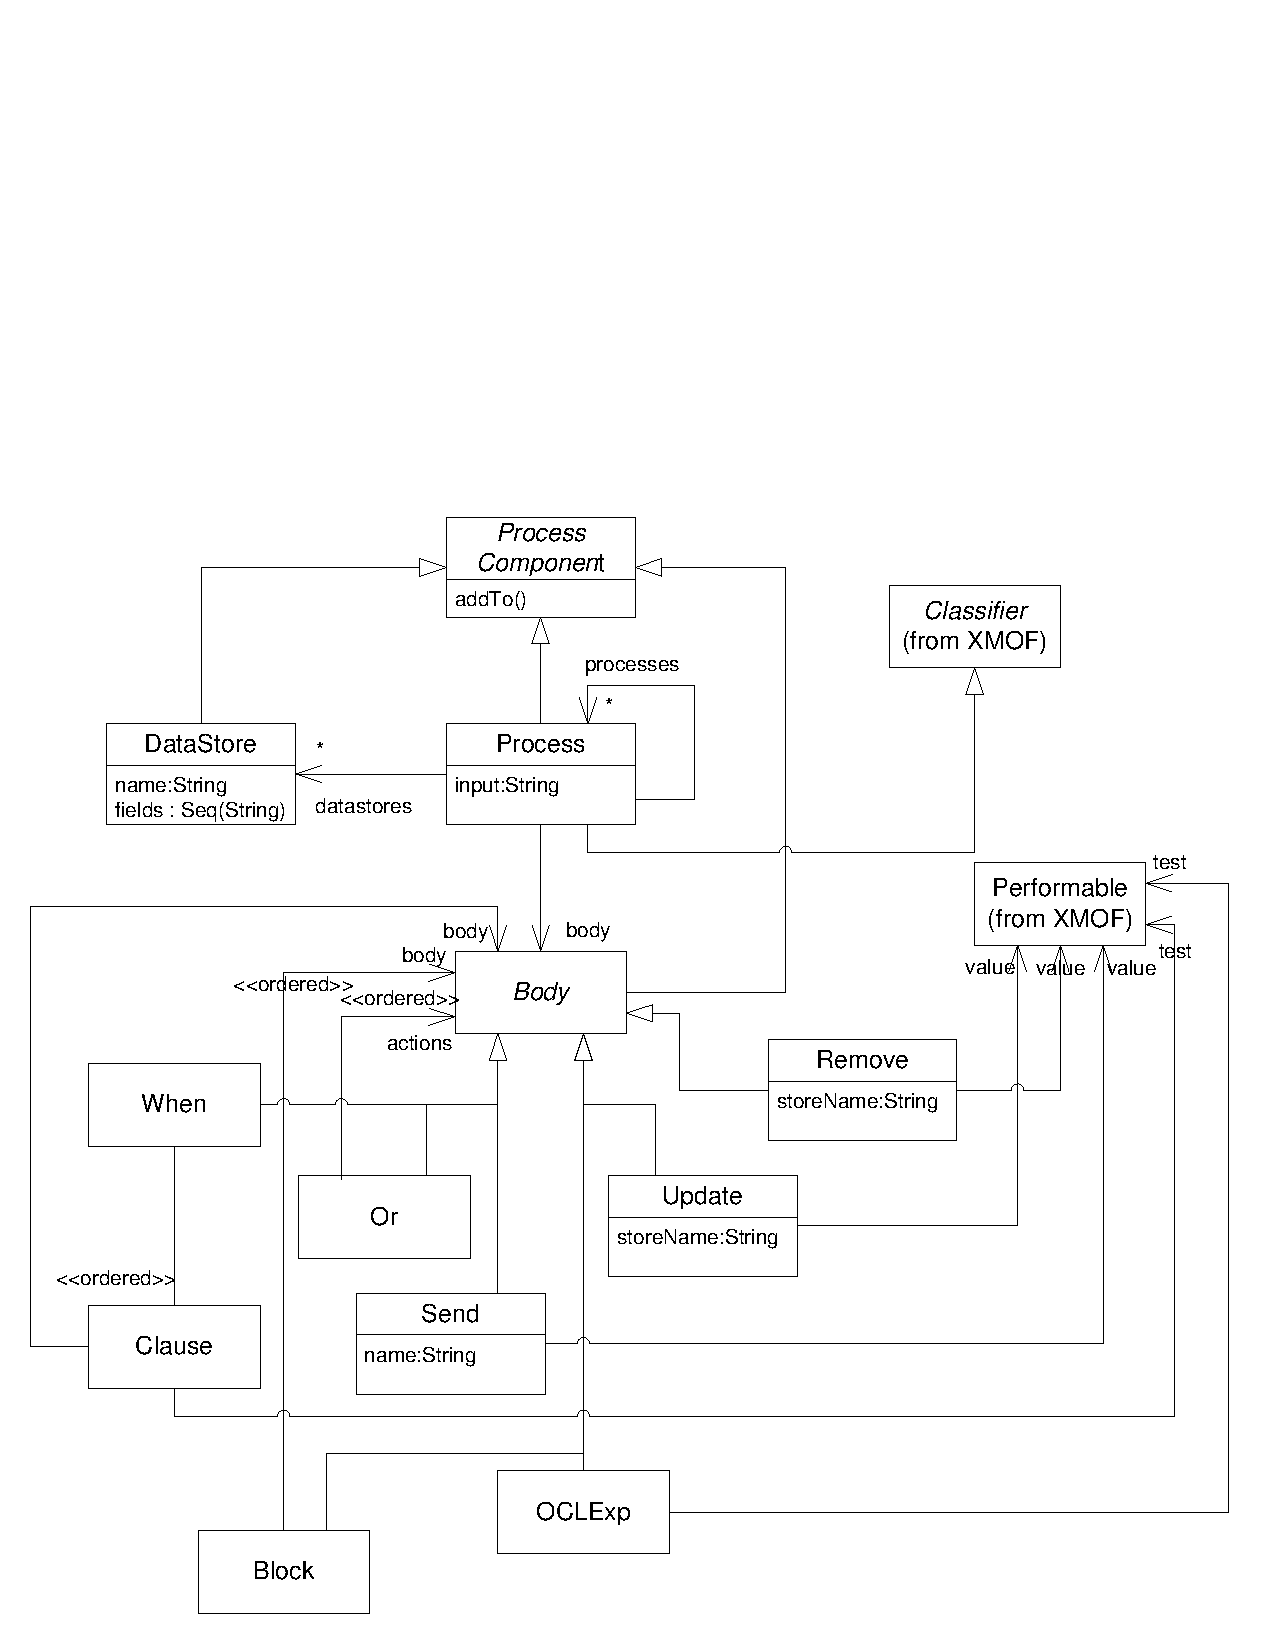
\includegraphics[width=12cm]{CaseStudy1/figures/DFDAbs2.pdf}
\caption{Abstract syntax model for DFDs} \label{dfdabs2}
\end{center}
\end{figure}

Note, the advantage of extension here is that ...

\subsection{Concrete Syntax}

\subsection{Semantic Domain}

In order to capture the semantics of process and datastore
instantiation, a semantic domain model needs to be constructed.
This is shown in figure \ref{dfdsem}:

\begin{figure}[htb]
\begin{center}
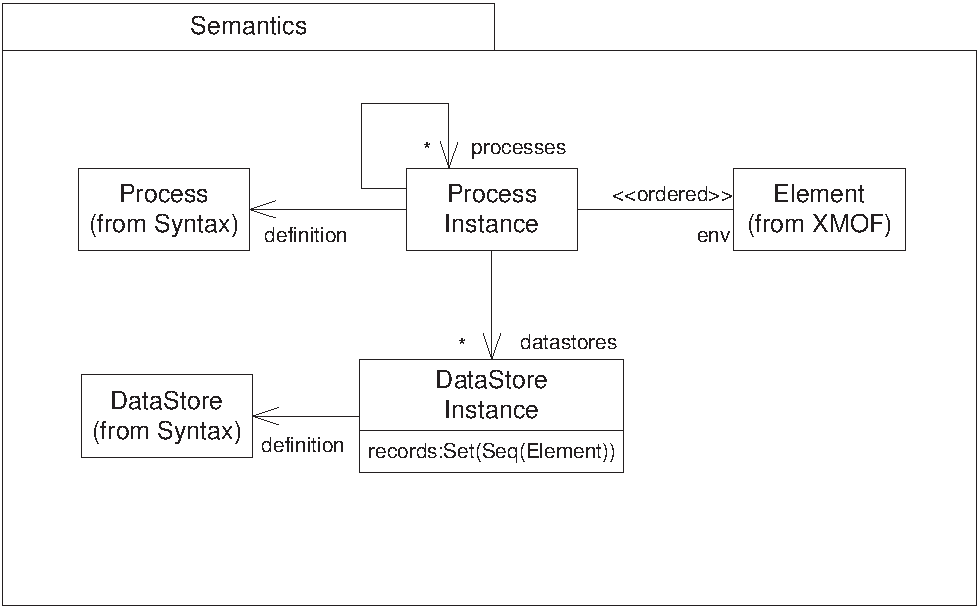
\includegraphics[width=12cm]{CaseStudy1/figures/DFDSem.pdf}
\caption{Semantic domain model for DFDs} \label{dfdsem}
\end{center}
\end{figure}

Now it possible to define what it means to create a new instance of
a process and a datastore. For a process, the following operation
is required, which is then called from the new() operation:

\begin{lstlisting}
context Root::DFD::Syntax::Process
  @Operation nestedNew(env:Element):Element
    let process = DFD::Semantics::Process.new();
        myProcessEnv = processes->collect(p |
          Seq{p.name})->asSeq; myStoreEnv = dataStores->collect(s |
            Seq{s.name})->asSeq
    in process.definition := self;
       process.processes := processes->collect(p |
         p.nestedNew(myProcessEnv + myStoreEnv + env));
       process.dataStores := dataStores->collect(s |
         s.new());
       @For pair in myProcessEnv do
         pair.tail := process.getProcess(pair->head)
       end;
       @For pair in myStoreEnv do
         pair.tail := process.getStore(pair->head)
       end;
       process.env := myProcessEnv + myStoreEnv + env
    end
  end
\end{lstlisting}where getProcess() and getStore returns the sub-processes and
stores associated with the process.

\section{Conclusion}
